% Created by tikzDevice version 0.12.4 on 2023-10-09 16:01:25
% !TEX encoding = UTF-8 Unicode
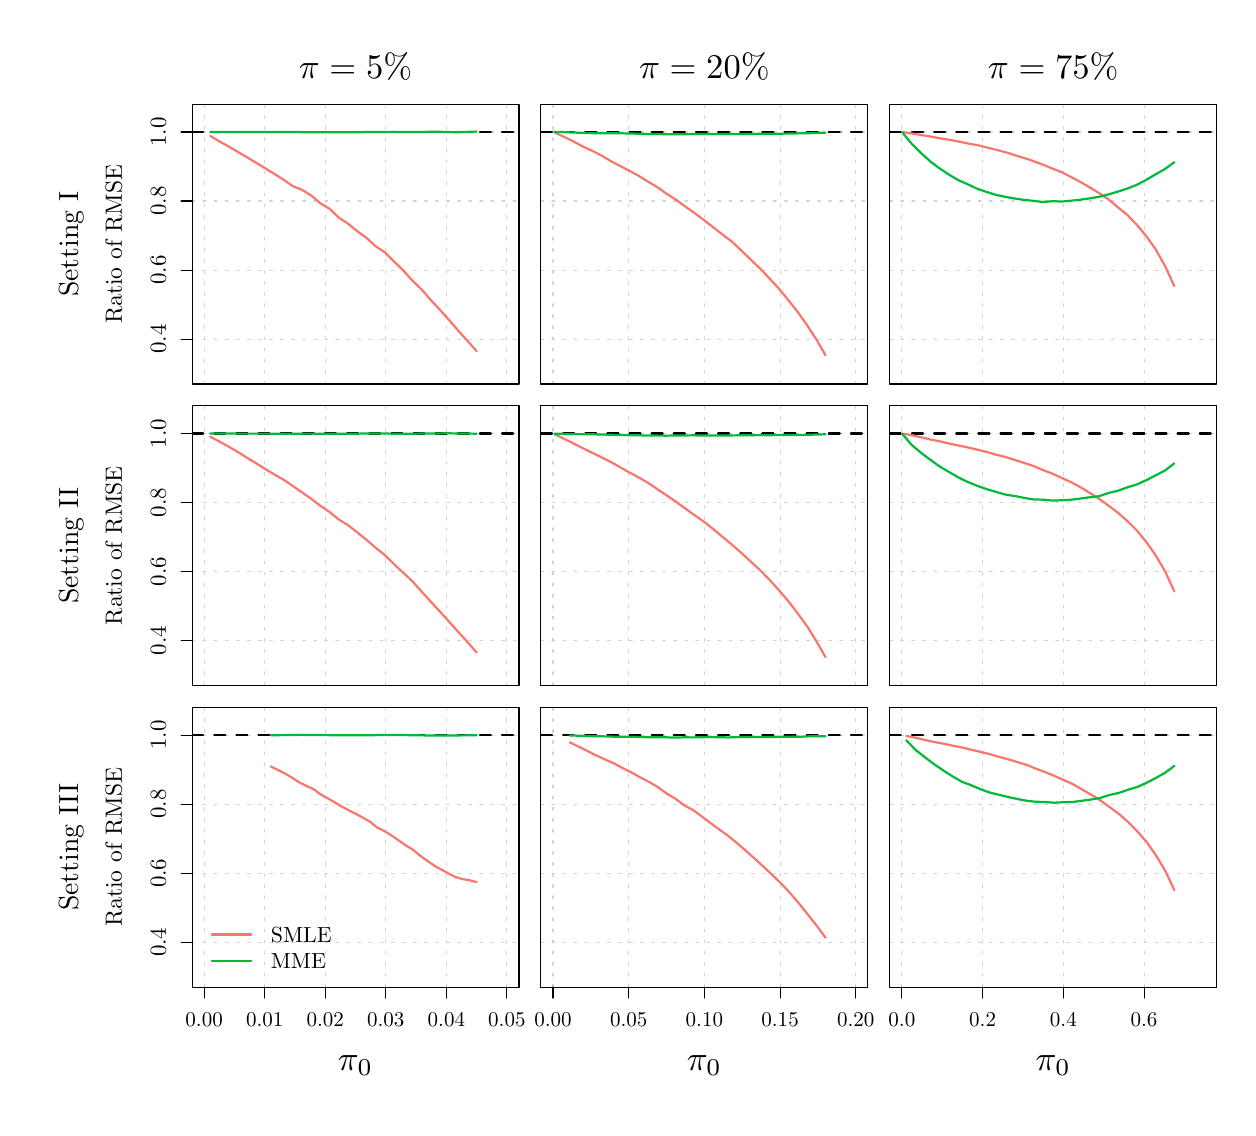
\begin{tikzpicture}[x=1pt,y=1pt]
\definecolor{fillColor}{RGB}{255,255,255}
\path[use as bounding box,fill=fillColor,fill opacity=0.00] (0,0) rectangle (433.62,390.26);
\begin{scope}
\path[clip] ( 55.44,257.53) rectangle (181.50,366.50);
\definecolor{drawColor}{RGB}{0,0,0}

\node[text=drawColor,anchor=base,inner sep=0pt, outer sep=0pt, scale=  0.66] at (118.47,231.40) {Simulation ID};

\node[text=drawColor,rotate= 90.00,anchor=base,inner sep=0pt, outer sep=0pt, scale=  0.66] at ( 34.06,312.01) {Ratio of RMSE};
\end{scope}
\begin{scope}
\path[clip] (  0.00,  0.00) rectangle (433.62,390.26);
\definecolor{drawColor}{RGB}{0,0,0}

\path[draw=drawColor,line width= 0.4pt,line join=round,line cap=round] ( 59.40,277.71) -- ( 59.40,352.56);

\path[draw=drawColor,line width= 0.4pt,line join=round,line cap=round] ( 59.40,277.71) -- ( 55.44,277.71);

\path[draw=drawColor,line width= 0.4pt,line join=round,line cap=round] ( 59.40,302.66) -- ( 55.44,302.66);

\path[draw=drawColor,line width= 0.4pt,line join=round,line cap=round] ( 59.40,327.61) -- ( 55.44,327.61);

\path[draw=drawColor,line width= 0.4pt,line join=round,line cap=round] ( 59.40,352.56) -- ( 55.44,352.56);

\node[text=drawColor,rotate= 90.00,anchor=base,inner sep=0pt, outer sep=0pt, scale=  0.83] at ( 49.90,277.71) {0.4};

\node[text=drawColor,rotate= 90.00,anchor=base,inner sep=0pt, outer sep=0pt, scale=  0.83] at ( 49.90,302.66) {0.6};

\node[text=drawColor,rotate= 90.00,anchor=base,inner sep=0pt, outer sep=0pt, scale=  0.83] at ( 49.90,327.61) {0.8};

\node[text=drawColor,rotate= 90.00,anchor=base,inner sep=0pt, outer sep=0pt, scale=  0.83] at ( 49.90,352.56) {1.0};
\end{scope}
\begin{scope}
\path[clip] ( 59.40,261.49) rectangle (177.54,362.54);
\definecolor{drawColor}{RGB}{211,211,211}

\path[draw=drawColor,line width= 0.4pt,dash pattern=on 1pt off 3pt ,line join=round,line cap=round] ( 63.78,261.49) -- ( 63.78,362.54);

\path[draw=drawColor,line width= 0.4pt,dash pattern=on 1pt off 3pt ,line join=round,line cap=round] ( 85.65,261.49) -- ( 85.65,362.54);

\path[draw=drawColor,line width= 0.4pt,dash pattern=on 1pt off 3pt ,line join=round,line cap=round] (107.53,261.49) -- (107.53,362.54);

\path[draw=drawColor,line width= 0.4pt,dash pattern=on 1pt off 3pt ,line join=round,line cap=round] (129.41,261.49) -- (129.41,362.54);

\path[draw=drawColor,line width= 0.4pt,dash pattern=on 1pt off 3pt ,line join=round,line cap=round] (151.29,261.49) -- (151.29,362.54);

\path[draw=drawColor,line width= 0.4pt,dash pattern=on 1pt off 3pt ,line join=round,line cap=round] (173.16,261.49) -- (173.16,362.54);

\path[draw=drawColor,line width= 0.4pt,dash pattern=on 1pt off 3pt ,line join=round,line cap=round] ( 59.40,277.71) -- (177.54,277.71);

\path[draw=drawColor,line width= 0.4pt,dash pattern=on 1pt off 3pt ,line join=round,line cap=round] ( 59.40,302.66) -- (177.54,302.66);

\path[draw=drawColor,line width= 0.4pt,dash pattern=on 1pt off 3pt ,line join=round,line cap=round] ( 59.40,327.61) -- (177.54,327.61);

\path[draw=drawColor,line width= 0.4pt,dash pattern=on 1pt off 3pt ,line join=round,line cap=round] ( 59.40,352.56) -- (177.54,352.56);
\end{scope}
\begin{scope}
\path[clip] (  0.00,  0.00) rectangle (433.62,390.26);
\definecolor{drawColor}{RGB}{0,0,0}

\path[draw=drawColor,line width= 0.4pt,line join=round,line cap=round] ( 59.40,261.49) --
	(177.54,261.49) --
	(177.54,362.54) --
	( 59.40,362.54) --
	cycle;
\end{scope}
\begin{scope}
\path[clip] ( 59.40,261.49) rectangle (177.54,362.54);
\definecolor{drawColor}{RGB}{0,0,0}

\path[draw=drawColor,line width= 0.8pt,dash pattern=on 4pt off 4pt ,line join=round,line cap=round] ( 59.40,352.56) -- (177.54,352.56);
\definecolor{drawColor}{RGB}{248,118,109}

\path[draw=drawColor,line width= 0.8pt,line join=round,line cap=round] ( 65.96,351.14) --
	( 69.28,349.16) --
	( 72.60,347.35) --
	( 75.92,345.40) --
	( 79.24,343.43) --
	( 82.56,341.42) --
	( 85.88,339.43) --
	( 89.20,337.38) --
	( 92.52,335.29) --
	( 95.84,332.96) --
	( 99.16,331.65) --
	(102.48,329.62) --
	(105.80,326.75) --
	(109.12,324.80) --
	(112.43,321.62) --
	(115.75,319.43) --
	(119.07,316.73) --
	(122.39,314.32) --
	(125.71,311.29) --
	(129.03,309.10) --
	(132.35,305.77) --
	(135.67,302.60) --
	(138.99,298.88) --
	(142.31,295.71) --
	(145.63,291.87) --
	(148.95,288.31) --
	(152.27,284.65) --
	(155.59,280.75) --
	(158.91,277.11) --
	(162.23,273.37);
\definecolor{drawColor}{RGB}{0,186,56}

\path[draw=drawColor,line width= 0.8pt,line join=round,line cap=round] ( 65.96,352.56) --
	( 69.28,352.56) --
	( 72.60,352.56) --
	( 75.92,352.58) --
	( 79.24,352.59) --
	( 82.56,352.58) --
	( 85.88,352.55) --
	( 89.20,352.55) --
	( 92.52,352.55) --
	( 95.84,352.57) --
	( 99.16,352.50) --
	(102.48,352.49) --
	(105.80,352.48) --
	(109.12,352.45) --
	(112.43,352.46) --
	(115.75,352.45) --
	(119.07,352.48) --
	(122.39,352.53) --
	(125.71,352.57) --
	(129.03,352.59) --
	(132.35,352.61) --
	(135.67,352.58) --
	(138.99,352.56) --
	(142.31,352.57) --
	(145.63,352.65) --
	(148.95,352.63) --
	(152.27,352.53) --
	(155.59,352.48) --
	(158.91,352.60) --
	(162.23,352.71);
\end{scope}
\begin{scope}
\path[clip] (  0.00,  0.00) rectangle (433.62,390.26);
\definecolor{drawColor}{RGB}{0,0,0}

\node[text=drawColor,rotate= 90.00,anchor=base,inner sep=0pt, outer sep=0pt, scale=  1.00] at ( 18.22,312.01) {Setting I};

\node[text=drawColor,rotate= 90.00,anchor=base,inner sep=0pt, outer sep=0pt, scale=  0.85] at ( 34.06,312.01) {Ratio of RMSE};

\node[text=drawColor,anchor=base,inner sep=0pt, outer sep=0pt, scale=  1.25] at (118.47,372.04) {$\pi = 5\%$};
\end{scope}
\begin{scope}
\path[clip] (181.50,257.53) rectangle (307.56,366.50);
\definecolor{drawColor}{RGB}{0,0,0}

\node[text=drawColor,anchor=base,inner sep=0pt, outer sep=0pt, scale=  0.66] at (244.53,231.40) {Simulation ID};

\node[text=drawColor,rotate= 90.00,anchor=base,inner sep=0pt, outer sep=0pt, scale=  0.66] at (160.12,312.01) {Ratio of RMSE};
\end{scope}
\begin{scope}
\path[clip] (185.46,261.49) rectangle (303.60,362.54);
\definecolor{drawColor}{RGB}{211,211,211}

\path[draw=drawColor,line width= 0.4pt,dash pattern=on 1pt off 3pt ,line join=round,line cap=round] (189.84,261.49) -- (189.84,362.54);

\path[draw=drawColor,line width= 0.4pt,dash pattern=on 1pt off 3pt ,line join=round,line cap=round] (217.18,261.49) -- (217.18,362.54);

\path[draw=drawColor,line width= 0.4pt,dash pattern=on 1pt off 3pt ,line join=round,line cap=round] (244.53,261.49) -- (244.53,362.54);

\path[draw=drawColor,line width= 0.4pt,dash pattern=on 1pt off 3pt ,line join=round,line cap=round] (271.88,261.49) -- (271.88,362.54);

\path[draw=drawColor,line width= 0.4pt,dash pattern=on 1pt off 3pt ,line join=round,line cap=round] (299.22,261.49) -- (299.22,362.54);

\path[draw=drawColor,line width= 0.4pt,dash pattern=on 1pt off 3pt ,line join=round,line cap=round] (185.46,277.71) -- (303.60,277.71);

\path[draw=drawColor,line width= 0.4pt,dash pattern=on 1pt off 3pt ,line join=round,line cap=round] (185.46,302.66) -- (303.60,302.66);

\path[draw=drawColor,line width= 0.4pt,dash pattern=on 1pt off 3pt ,line join=round,line cap=round] (185.46,327.61) -- (303.60,327.61);

\path[draw=drawColor,line width= 0.4pt,dash pattern=on 1pt off 3pt ,line join=round,line cap=round] (185.46,352.56) -- (303.60,352.56);
\end{scope}
\begin{scope}
\path[clip] (  0.00,  0.00) rectangle (433.62,390.26);
\definecolor{drawColor}{RGB}{0,0,0}

\path[draw=drawColor,line width= 0.4pt,line join=round,line cap=round] (185.46,261.49) --
	(303.60,261.49) --
	(303.60,362.54) --
	(185.46,362.54) --
	cycle;
\end{scope}
\begin{scope}
\path[clip] (185.46,261.49) rectangle (303.60,362.54);
\definecolor{drawColor}{RGB}{0,0,0}

\path[draw=drawColor,line width= 0.8pt,dash pattern=on 4pt off 4pt ,line join=round,line cap=round] (185.46,352.56) -- (303.60,352.56);
\definecolor{drawColor}{RGB}{248,118,109}

\path[draw=drawColor,line width= 0.8pt,line join=round,line cap=round] (190.38,352.40) --
	(193.76,350.83) --
	(197.13,349.20) --
	(200.51,347.37) --
	(203.89,345.80) --
	(207.26,344.10) --
	(210.64,342.07) --
	(214.01,340.30) --
	(217.39,338.57) --
	(220.77,336.73) --
	(224.14,334.62) --
	(227.52,332.63) --
	(230.89,330.23) --
	(234.27,328.08) --
	(237.65,325.60) --
	(241.02,323.25) --
	(244.40,320.68) --
	(247.77,318.10) --
	(251.15,315.47) --
	(254.53,312.90) --
	(257.90,309.71) --
	(261.28,306.42) --
	(264.65,303.25) --
	(268.03,299.66) --
	(271.41,296.03) --
	(274.78,291.90) --
	(278.16,287.67) --
	(281.53,282.92) --
	(284.91,277.73) --
	(288.29,271.92);
\definecolor{drawColor}{RGB}{0,186,56}

\path[draw=drawColor,line width= 0.8pt,line join=round,line cap=round] (190.38,352.62) --
	(193.76,352.51) --
	(197.13,352.36) --
	(200.51,352.25) --
	(203.89,352.14) --
	(207.26,352.11) --
	(210.64,352.11) --
	(214.01,352.09) --
	(217.39,352.03) --
	(220.77,351.93) --
	(224.14,351.85) --
	(227.52,351.82) --
	(230.89,351.76) --
	(234.27,351.70) --
	(237.65,351.77) --
	(241.02,351.83) --
	(244.40,351.85) --
	(247.77,351.80) --
	(251.15,351.80) --
	(254.53,351.81) --
	(257.90,351.81) --
	(261.28,351.84) --
	(264.65,351.91) --
	(268.03,351.94) --
	(271.41,351.95) --
	(274.78,351.98) --
	(278.16,352.06) --
	(281.53,352.10) --
	(284.91,352.20) --
	(288.29,352.33);
\end{scope}
\begin{scope}
\path[clip] (  0.00,  0.00) rectangle (433.62,390.26);
\definecolor{drawColor}{RGB}{0,0,0}

\node[text=drawColor,anchor=base,inner sep=0pt, outer sep=0pt, scale=  1.25] at (244.53,372.04) {$\pi = 20\%$};
\end{scope}
\begin{scope}
\path[clip] (307.56,257.53) rectangle (433.62,366.50);
\definecolor{drawColor}{RGB}{0,0,0}

\node[text=drawColor,anchor=base,inner sep=0pt, outer sep=0pt, scale=  0.66] at (370.59,231.40) {Simulation ID};

\node[text=drawColor,rotate= 90.00,anchor=base,inner sep=0pt, outer sep=0pt, scale=  0.66] at (286.18,312.01) {Ratio of RMSE};
\end{scope}
\begin{scope}
\path[clip] (311.52,261.49) rectangle (429.66,362.54);
\definecolor{drawColor}{RGB}{211,211,211}

\path[draw=drawColor,line width= 0.4pt,dash pattern=on 1pt off 3pt ,line join=round,line cap=round] (315.90,261.49) -- (315.90,362.54);

\path[draw=drawColor,line width= 0.4pt,dash pattern=on 1pt off 3pt ,line join=round,line cap=round] (345.07,261.49) -- (345.07,362.54);

\path[draw=drawColor,line width= 0.4pt,dash pattern=on 1pt off 3pt ,line join=round,line cap=round] (374.24,261.49) -- (374.24,362.54);

\path[draw=drawColor,line width= 0.4pt,dash pattern=on 1pt off 3pt ,line join=round,line cap=round] (403.41,261.49) -- (403.41,362.54);

\path[draw=drawColor,line width= 0.4pt,dash pattern=on 1pt off 3pt ,line join=round,line cap=round] (311.52,277.71) -- (429.66,277.71);

\path[draw=drawColor,line width= 0.4pt,dash pattern=on 1pt off 3pt ,line join=round,line cap=round] (311.52,302.66) -- (429.66,302.66);

\path[draw=drawColor,line width= 0.4pt,dash pattern=on 1pt off 3pt ,line join=round,line cap=round] (311.52,327.61) -- (429.66,327.61);

\path[draw=drawColor,line width= 0.4pt,dash pattern=on 1pt off 3pt ,line join=round,line cap=round] (311.52,352.56) -- (429.66,352.56);
\end{scope}
\begin{scope}
\path[clip] (  0.00,  0.00) rectangle (433.62,390.26);
\definecolor{drawColor}{RGB}{0,0,0}

\path[draw=drawColor,line width= 0.4pt,line join=round,line cap=round] (311.52,261.49) --
	(429.66,261.49) --
	(429.66,362.54) --
	(311.52,362.54) --
	cycle;
\end{scope}
\begin{scope}
\path[clip] (311.52,261.49) rectangle (429.66,362.54);
\definecolor{drawColor}{RGB}{0,0,0}

\path[draw=drawColor,line width= 0.8pt,dash pattern=on 4pt off 4pt ,line join=round,line cap=round] (311.52,352.56) -- (429.66,352.56);
\definecolor{drawColor}{RGB}{248,118,109}

\path[draw=drawColor,line width= 0.8pt,line join=round,line cap=round] (316.04,352.56) --
	(319.43,352.03) --
	(322.82,351.47) --
	(326.21,350.91) --
	(329.60,350.29) --
	(332.99,349.75) --
	(336.38,349.12) --
	(339.77,348.41) --
	(343.16,347.81) --
	(346.55,346.97) --
	(349.94,346.15) --
	(353.33,345.24) --
	(356.72,344.19) --
	(360.11,343.14) --
	(363.50,342.01) --
	(366.89,340.76) --
	(370.28,339.36) --
	(373.67,338.02) --
	(377.06,336.29) --
	(380.45,334.46) --
	(383.84,332.51) --
	(387.23,330.44) --
	(390.62,328.15) --
	(394.01,325.31) --
	(397.40,322.53) --
	(400.79,319.03) --
	(404.18,314.96) --
	(407.57,310.22) --
	(410.96,304.17) --
	(414.35,296.84);
\definecolor{drawColor}{RGB}{0,186,56}

\path[draw=drawColor,line width= 0.8pt,line join=round,line cap=round] (316.04,352.42) --
	(319.43,348.31) --
	(322.82,344.96) --
	(326.21,341.86) --
	(329.60,339.34) --
	(332.99,337.11) --
	(336.38,335.11) --
	(339.77,333.63) --
	(343.16,332.01) --
	(346.55,330.88) --
	(349.94,329.83) --
	(353.33,329.11) --
	(356.72,328.51) --
	(360.11,328.01) --
	(363.50,327.67) --
	(366.89,327.26) --
	(370.28,327.55) --
	(373.67,327.43) --
	(377.06,327.73) --
	(380.45,328.10) --
	(383.84,328.59) --
	(387.23,329.15) --
	(390.62,330.03) --
	(394.01,331.04) --
	(397.40,332.13) --
	(400.79,333.47) --
	(404.18,335.26) --
	(407.57,337.27) --
	(410.96,339.19) --
	(414.35,341.64);
\end{scope}
\begin{scope}
\path[clip] (  0.00,  0.00) rectangle (433.62,390.26);
\definecolor{drawColor}{RGB}{0,0,0}

\node[text=drawColor,anchor=base,inner sep=0pt, outer sep=0pt, scale=  1.25] at (370.59,372.04) {$\pi = 75\%$};
\end{scope}
\begin{scope}
\path[clip] ( 55.44,148.57) rectangle (181.50,257.53);
\definecolor{drawColor}{RGB}{0,0,0}

\node[text=drawColor,anchor=base,inner sep=0pt, outer sep=0pt, scale=  0.66] at (118.47,122.43) {Simulation ID};

\node[text=drawColor,rotate= 90.00,anchor=base,inner sep=0pt, outer sep=0pt, scale=  0.66] at ( 34.06,203.05) {Ratio of RMSE};
\end{scope}
\begin{scope}
\path[clip] (  0.00,  0.00) rectangle (433.62,390.26);
\definecolor{drawColor}{RGB}{0,0,0}

\path[draw=drawColor,line width= 0.4pt,line join=round,line cap=round] ( 59.40,168.74) -- ( 59.40,243.59);

\path[draw=drawColor,line width= 0.4pt,line join=round,line cap=round] ( 59.40,168.74) -- ( 55.44,168.74);

\path[draw=drawColor,line width= 0.4pt,line join=round,line cap=round] ( 59.40,193.69) -- ( 55.44,193.69);

\path[draw=drawColor,line width= 0.4pt,line join=round,line cap=round] ( 59.40,218.64) -- ( 55.44,218.64);

\path[draw=drawColor,line width= 0.4pt,line join=round,line cap=round] ( 59.40,243.59) -- ( 55.44,243.59);

\node[text=drawColor,rotate= 90.00,anchor=base,inner sep=0pt, outer sep=0pt, scale=  0.83] at ( 49.90,168.74) {0.4};

\node[text=drawColor,rotate= 90.00,anchor=base,inner sep=0pt, outer sep=0pt, scale=  0.83] at ( 49.90,193.69) {0.6};

\node[text=drawColor,rotate= 90.00,anchor=base,inner sep=0pt, outer sep=0pt, scale=  0.83] at ( 49.90,218.64) {0.8};

\node[text=drawColor,rotate= 90.00,anchor=base,inner sep=0pt, outer sep=0pt, scale=  0.83] at ( 49.90,243.59) {1.0};
\end{scope}
\begin{scope}
\path[clip] ( 59.40,152.53) rectangle (177.54,253.57);
\definecolor{drawColor}{RGB}{211,211,211}

\path[draw=drawColor,line width= 0.4pt,dash pattern=on 1pt off 3pt ,line join=round,line cap=round] ( 63.78,152.53) -- ( 63.78,253.57);

\path[draw=drawColor,line width= 0.4pt,dash pattern=on 1pt off 3pt ,line join=round,line cap=round] ( 85.65,152.53) -- ( 85.65,253.57);

\path[draw=drawColor,line width= 0.4pt,dash pattern=on 1pt off 3pt ,line join=round,line cap=round] (107.53,152.53) -- (107.53,253.57);

\path[draw=drawColor,line width= 0.4pt,dash pattern=on 1pt off 3pt ,line join=round,line cap=round] (129.41,152.53) -- (129.41,253.57);

\path[draw=drawColor,line width= 0.4pt,dash pattern=on 1pt off 3pt ,line join=round,line cap=round] (151.29,152.53) -- (151.29,253.57);

\path[draw=drawColor,line width= 0.4pt,dash pattern=on 1pt off 3pt ,line join=round,line cap=round] (173.16,152.53) -- (173.16,253.57);

\path[draw=drawColor,line width= 0.4pt,dash pattern=on 1pt off 3pt ,line join=round,line cap=round] ( 59.40,168.74) -- (177.54,168.74);

\path[draw=drawColor,line width= 0.4pt,dash pattern=on 1pt off 3pt ,line join=round,line cap=round] ( 59.40,193.69) -- (177.54,193.69);

\path[draw=drawColor,line width= 0.4pt,dash pattern=on 1pt off 3pt ,line join=round,line cap=round] ( 59.40,218.64) -- (177.54,218.64);

\path[draw=drawColor,line width= 0.4pt,dash pattern=on 1pt off 3pt ,line join=round,line cap=round] ( 59.40,243.59) -- (177.54,243.59);
\end{scope}
\begin{scope}
\path[clip] (  0.00,  0.00) rectangle (433.62,390.26);
\definecolor{drawColor}{RGB}{0,0,0}

\path[draw=drawColor,line width= 0.4pt,line join=round,line cap=round] ( 59.40,152.53) --
	(177.54,152.53) --
	(177.54,253.57) --
	( 59.40,253.57) --
	cycle;
\end{scope}
\begin{scope}
\path[clip] ( 59.40,152.53) rectangle (177.54,253.57);
\definecolor{drawColor}{RGB}{0,0,0}

\path[draw=drawColor,line width= 0.8pt,dash pattern=on 4pt off 4pt ,line join=round,line cap=round] ( 59.40,243.59) -- (177.54,243.59);
\definecolor{drawColor}{RGB}{248,118,109}

\path[draw=drawColor,line width= 0.8pt,line join=round,line cap=round] ( 65.96,242.43) --
	( 69.28,240.72) --
	( 72.60,238.86) --
	( 75.92,236.97) --
	( 79.24,234.86) --
	( 82.56,232.84) --
	( 85.88,230.77) --
	( 89.20,228.75) --
	( 92.52,226.89) --
	( 95.84,224.62) --
	( 99.16,222.32) --
	(102.48,220.00) --
	(105.80,217.46) --
	(109.12,215.23) --
	(112.43,212.53) --
	(115.75,210.48) --
	(119.07,207.92) --
	(122.39,205.21) --
	(125.71,202.34) --
	(129.03,199.72) --
	(132.35,196.42) --
	(135.67,193.32) --
	(138.99,190.25) --
	(142.31,186.55) --
	(145.63,182.85) --
	(148.95,179.29) --
	(152.27,175.62) --
	(155.59,171.90) --
	(158.91,168.30) --
	(162.23,164.47);
\definecolor{drawColor}{RGB}{0,186,56}

\path[draw=drawColor,line width= 0.8pt,line join=round,line cap=round] ( 65.96,243.61) --
	( 69.28,243.60) --
	( 72.60,243.59) --
	( 75.92,243.57) --
	( 79.24,243.57) --
	( 82.56,243.57) --
	( 85.88,243.57) --
	( 89.20,243.55) --
	( 92.52,243.54) --
	( 95.84,243.54) --
	( 99.16,243.56) --
	(102.48,243.56) --
	(105.80,243.55) --
	(109.12,243.51) --
	(112.43,243.51) --
	(115.75,243.52) --
	(119.07,243.56) --
	(122.39,243.60) --
	(125.71,243.62) --
	(129.03,243.59) --
	(132.35,243.55) --
	(135.67,243.55) --
	(138.99,243.55) --
	(142.31,243.58) --
	(145.63,243.62) --
	(148.95,243.65) --
	(152.27,243.68) --
	(155.59,243.62) --
	(158.91,243.59) --
	(162.23,243.54);
\end{scope}
\begin{scope}
\path[clip] (  0.00,  0.00) rectangle (433.62,390.26);
\definecolor{drawColor}{RGB}{0,0,0}

\node[text=drawColor,rotate= 90.00,anchor=base,inner sep=0pt, outer sep=0pt, scale=  1.00] at ( 18.22,203.05) {Setting II};

\node[text=drawColor,rotate= 90.00,anchor=base,inner sep=0pt, outer sep=0pt, scale=  0.85] at ( 34.06,203.05) {Ratio of RMSE};
\end{scope}
\begin{scope}
\path[clip] (181.50,148.57) rectangle (307.56,257.53);
\definecolor{drawColor}{RGB}{0,0,0}

\node[text=drawColor,anchor=base,inner sep=0pt, outer sep=0pt, scale=  0.66] at (244.53,122.43) {Simulation ID};

\node[text=drawColor,rotate= 90.00,anchor=base,inner sep=0pt, outer sep=0pt, scale=  0.66] at (160.12,203.05) {Ratio of RMSE};
\end{scope}
\begin{scope}
\path[clip] (185.46,152.53) rectangle (303.60,253.57);
\definecolor{drawColor}{RGB}{211,211,211}

\path[draw=drawColor,line width= 0.4pt,dash pattern=on 1pt off 3pt ,line join=round,line cap=round] (189.84,152.53) -- (189.84,253.57);

\path[draw=drawColor,line width= 0.4pt,dash pattern=on 1pt off 3pt ,line join=round,line cap=round] (217.18,152.53) -- (217.18,253.57);

\path[draw=drawColor,line width= 0.4pt,dash pattern=on 1pt off 3pt ,line join=round,line cap=round] (244.53,152.53) -- (244.53,253.57);

\path[draw=drawColor,line width= 0.4pt,dash pattern=on 1pt off 3pt ,line join=round,line cap=round] (271.88,152.53) -- (271.88,253.57);

\path[draw=drawColor,line width= 0.4pt,dash pattern=on 1pt off 3pt ,line join=round,line cap=round] (299.22,152.53) -- (299.22,253.57);

\path[draw=drawColor,line width= 0.4pt,dash pattern=on 1pt off 3pt ,line join=round,line cap=round] (185.46,168.74) -- (303.60,168.74);

\path[draw=drawColor,line width= 0.4pt,dash pattern=on 1pt off 3pt ,line join=round,line cap=round] (185.46,193.69) -- (303.60,193.69);

\path[draw=drawColor,line width= 0.4pt,dash pattern=on 1pt off 3pt ,line join=round,line cap=round] (185.46,218.64) -- (303.60,218.64);

\path[draw=drawColor,line width= 0.4pt,dash pattern=on 1pt off 3pt ,line join=round,line cap=round] (185.46,243.59) -- (303.60,243.59);
\end{scope}
\begin{scope}
\path[clip] (  0.00,  0.00) rectangle (433.62,390.26);
\definecolor{drawColor}{RGB}{0,0,0}

\path[draw=drawColor,line width= 0.4pt,line join=round,line cap=round] (185.46,152.53) --
	(303.60,152.53) --
	(303.60,253.57) --
	(185.46,253.57) --
	cycle;
\end{scope}
\begin{scope}
\path[clip] (185.46,152.53) rectangle (303.60,253.57);
\definecolor{drawColor}{RGB}{0,0,0}

\path[draw=drawColor,line width= 0.8pt,dash pattern=on 4pt off 4pt ,line join=round,line cap=round] (185.46,243.59) -- (303.60,243.59);
\definecolor{drawColor}{RGB}{248,118,109}

\path[draw=drawColor,line width= 0.8pt,line join=round,line cap=round] (190.38,243.32) --
	(193.76,241.73) --
	(197.13,240.06) --
	(200.51,238.35) --
	(203.89,236.71) --
	(207.26,235.04) --
	(210.64,233.35) --
	(214.01,231.47) --
	(217.39,229.55) --
	(220.77,227.73) --
	(224.14,225.79) --
	(227.52,223.51) --
	(230.89,221.24) --
	(234.27,218.95) --
	(237.65,216.49) --
	(241.02,214.05) --
	(244.40,211.72) --
	(247.77,209.04) --
	(251.15,206.21) --
	(254.53,203.41) --
	(257.90,200.47) --
	(261.28,197.32) --
	(264.65,194.23) --
	(268.03,190.76) --
	(271.41,187.04) --
	(274.78,183.12) --
	(278.16,178.72) --
	(281.53,174.14) --
	(284.91,168.69) --
	(288.29,162.82);
\definecolor{drawColor}{RGB}{0,186,56}

\path[draw=drawColor,line width= 0.8pt,line join=round,line cap=round] (190.38,243.56) --
	(193.76,243.47) --
	(197.13,243.40) --
	(200.51,243.38) --
	(203.89,243.32) --
	(207.26,243.26) --
	(210.64,243.15) --
	(214.01,243.05) --
	(217.39,243.01) --
	(220.77,242.95) --
	(224.14,242.88) --
	(227.52,242.85) --
	(230.89,242.83) --
	(234.27,242.89) --
	(237.65,242.92) --
	(241.02,242.95) --
	(244.40,242.85) --
	(247.77,242.87) --
	(251.15,242.91) --
	(254.53,242.92) --
	(257.90,242.97) --
	(261.28,243.00) --
	(264.65,243.03) --
	(268.03,243.00) --
	(271.41,243.06) --
	(274.78,243.07) --
	(278.16,243.11) --
	(281.53,243.11) --
	(284.91,243.24) --
	(288.29,243.33);
\end{scope}
\begin{scope}
\path[clip] (307.56,148.57) rectangle (433.62,257.53);
\definecolor{drawColor}{RGB}{0,0,0}

\node[text=drawColor,anchor=base,inner sep=0pt, outer sep=0pt, scale=  0.66] at (370.59,122.43) {Simulation ID};

\node[text=drawColor,rotate= 90.00,anchor=base,inner sep=0pt, outer sep=0pt, scale=  0.66] at (286.18,203.05) {Ratio of RMSE};
\end{scope}
\begin{scope}
\path[clip] (311.52,152.53) rectangle (429.66,253.57);
\definecolor{drawColor}{RGB}{211,211,211}

\path[draw=drawColor,line width= 0.4pt,dash pattern=on 1pt off 3pt ,line join=round,line cap=round] (315.90,152.53) -- (315.90,253.57);

\path[draw=drawColor,line width= 0.4pt,dash pattern=on 1pt off 3pt ,line join=round,line cap=round] (345.07,152.53) -- (345.07,253.57);

\path[draw=drawColor,line width= 0.4pt,dash pattern=on 1pt off 3pt ,line join=round,line cap=round] (374.24,152.53) -- (374.24,253.57);

\path[draw=drawColor,line width= 0.4pt,dash pattern=on 1pt off 3pt ,line join=round,line cap=round] (403.41,152.53) -- (403.41,253.57);

\path[draw=drawColor,line width= 0.4pt,dash pattern=on 1pt off 3pt ,line join=round,line cap=round] (311.52,168.74) -- (429.66,168.74);

\path[draw=drawColor,line width= 0.4pt,dash pattern=on 1pt off 3pt ,line join=round,line cap=round] (311.52,193.69) -- (429.66,193.69);

\path[draw=drawColor,line width= 0.4pt,dash pattern=on 1pt off 3pt ,line join=round,line cap=round] (311.52,218.64) -- (429.66,218.64);

\path[draw=drawColor,line width= 0.4pt,dash pattern=on 1pt off 3pt ,line join=round,line cap=round] (311.52,243.59) -- (429.66,243.59);
\end{scope}
\begin{scope}
\path[clip] (  0.00,  0.00) rectangle (433.62,390.26);
\definecolor{drawColor}{RGB}{0,0,0}

\path[draw=drawColor,line width= 0.4pt,line join=round,line cap=round] (311.52,152.53) --
	(429.66,152.53) --
	(429.66,253.57) --
	(311.52,253.57) --
	cycle;
\end{scope}
\begin{scope}
\path[clip] (311.52,152.53) rectangle (429.66,253.57);
\definecolor{drawColor}{RGB}{0,0,0}

\path[draw=drawColor,line width= 0.8pt,dash pattern=on 4pt off 4pt ,line join=round,line cap=round] (311.52,243.59) -- (429.66,243.59);
\definecolor{drawColor}{RGB}{248,118,109}

\path[draw=drawColor,line width= 0.8pt,line join=round,line cap=round] (316.04,243.57) --
	(319.43,243.01) --
	(322.82,242.26) --
	(326.21,241.43) --
	(329.60,240.79) --
	(332.99,239.96) --
	(336.38,239.27) --
	(339.77,238.56) --
	(343.16,237.77) --
	(346.55,236.95) --
	(349.94,235.95) --
	(353.33,235.12) --
	(356.72,234.03) --
	(360.11,232.97) --
	(363.50,231.86) --
	(366.89,230.38) --
	(370.28,229.12) --
	(373.67,227.54) --
	(377.06,226.03) --
	(380.45,224.19) --
	(383.84,222.10) --
	(387.23,219.99) --
	(390.62,217.48) --
	(394.01,214.94) --
	(397.40,211.94) --
	(400.79,208.58) --
	(404.18,204.45) --
	(407.57,199.63) --
	(410.96,193.89) --
	(414.35,186.56);
\definecolor{drawColor}{RGB}{0,186,56}

\path[draw=drawColor,line width= 0.8pt,line join=round,line cap=round] (316.04,243.44) --
	(319.43,239.48) --
	(322.82,236.63) --
	(326.21,234.09) --
	(329.60,231.64) --
	(332.99,229.68) --
	(336.38,227.71) --
	(339.77,226.05) --
	(343.16,224.70) --
	(346.55,223.49) --
	(349.94,222.49) --
	(353.33,221.53) --
	(356.72,221.01) --
	(360.11,220.34) --
	(363.50,219.76) --
	(366.89,219.70) --
	(370.28,219.38) --
	(373.67,219.48) --
	(377.06,219.68) --
	(380.45,220.10) --
	(383.84,220.58) --
	(387.23,220.97) --
	(390.62,222.16) --
	(394.01,222.93) --
	(397.40,224.17) --
	(400.79,225.20) --
	(404.18,226.74) --
	(407.57,228.47) --
	(410.96,230.24) --
	(414.35,232.84);
\end{scope}
\begin{scope}
\path[clip] ( 55.44, 39.60) rectangle (181.50,148.57);
\definecolor{drawColor}{RGB}{0,0,0}

\node[text=drawColor,anchor=base,inner sep=0pt, outer sep=0pt, scale=  0.66] at (118.47, 13.46) {Simulation ID};

\node[text=drawColor,rotate= 90.00,anchor=base,inner sep=0pt, outer sep=0pt, scale=  0.66] at ( 34.06, 94.08) {Ratio of RMSE};
\end{scope}
\begin{scope}
\path[clip] (  0.00,  0.00) rectangle (433.62,390.26);
\definecolor{drawColor}{RGB}{0,0,0}

\path[draw=drawColor,line width= 0.4pt,line join=round,line cap=round] ( 59.40, 59.78) -- ( 59.40,134.63);

\path[draw=drawColor,line width= 0.4pt,line join=round,line cap=round] ( 59.40, 59.78) -- ( 55.44, 59.78);

\path[draw=drawColor,line width= 0.4pt,line join=round,line cap=round] ( 59.40, 84.73) -- ( 55.44, 84.73);

\path[draw=drawColor,line width= 0.4pt,line join=round,line cap=round] ( 59.40,109.68) -- ( 55.44,109.68);

\path[draw=drawColor,line width= 0.4pt,line join=round,line cap=round] ( 59.40,134.63) -- ( 55.44,134.63);

\node[text=drawColor,rotate= 90.00,anchor=base,inner sep=0pt, outer sep=0pt, scale=  0.83] at ( 49.90, 59.78) {0.4};

\node[text=drawColor,rotate= 90.00,anchor=base,inner sep=0pt, outer sep=0pt, scale=  0.83] at ( 49.90, 84.73) {0.6};

\node[text=drawColor,rotate= 90.00,anchor=base,inner sep=0pt, outer sep=0pt, scale=  0.83] at ( 49.90,109.68) {0.8};

\node[text=drawColor,rotate= 90.00,anchor=base,inner sep=0pt, outer sep=0pt, scale=  0.83] at ( 49.90,134.63) {1.0};
\end{scope}
\begin{scope}
\path[clip] ( 59.40, 43.56) rectangle (177.54,144.61);
\definecolor{drawColor}{RGB}{211,211,211}

\path[draw=drawColor,line width= 0.4pt,dash pattern=on 1pt off 3pt ,line join=round,line cap=round] ( 63.78, 43.56) -- ( 63.78,144.61);

\path[draw=drawColor,line width= 0.4pt,dash pattern=on 1pt off 3pt ,line join=round,line cap=round] ( 85.65, 43.56) -- ( 85.65,144.61);

\path[draw=drawColor,line width= 0.4pt,dash pattern=on 1pt off 3pt ,line join=round,line cap=round] (107.53, 43.56) -- (107.53,144.61);

\path[draw=drawColor,line width= 0.4pt,dash pattern=on 1pt off 3pt ,line join=round,line cap=round] (129.41, 43.56) -- (129.41,144.61);

\path[draw=drawColor,line width= 0.4pt,dash pattern=on 1pt off 3pt ,line join=round,line cap=round] (151.29, 43.56) -- (151.29,144.61);

\path[draw=drawColor,line width= 0.4pt,dash pattern=on 1pt off 3pt ,line join=round,line cap=round] (173.16, 43.56) -- (173.16,144.61);

\path[draw=drawColor,line width= 0.4pt,dash pattern=on 1pt off 3pt ,line join=round,line cap=round] ( 59.40, 59.78) -- (177.54, 59.78);

\path[draw=drawColor,line width= 0.4pt,dash pattern=on 1pt off 3pt ,line join=round,line cap=round] ( 59.40, 84.73) -- (177.54, 84.73);

\path[draw=drawColor,line width= 0.4pt,dash pattern=on 1pt off 3pt ,line join=round,line cap=round] ( 59.40,109.68) -- (177.54,109.68);

\path[draw=drawColor,line width= 0.4pt,dash pattern=on 1pt off 3pt ,line join=round,line cap=round] ( 59.40,134.63) -- (177.54,134.63);
\end{scope}
\begin{scope}
\path[clip] (  0.00,  0.00) rectangle (433.62,390.26);
\definecolor{drawColor}{RGB}{0,0,0}

\path[draw=drawColor,line width= 0.4pt,line join=round,line cap=round] ( 59.40, 43.56) --
	(177.54, 43.56) --
	(177.54,144.61) --
	( 59.40,144.61) --
	cycle;

\path[draw=drawColor,line width= 0.4pt,line join=round,line cap=round] ( 63.78, 43.56) -- (173.16, 43.56);

\path[draw=drawColor,line width= 0.4pt,line join=round,line cap=round] ( 63.78, 43.56) -- ( 63.78, 39.60);

\path[draw=drawColor,line width= 0.4pt,line join=round,line cap=round] ( 85.65, 43.56) -- ( 85.65, 39.60);

\path[draw=drawColor,line width= 0.4pt,line join=round,line cap=round] (107.53, 43.56) -- (107.53, 39.60);

\path[draw=drawColor,line width= 0.4pt,line join=round,line cap=round] (129.41, 43.56) -- (129.41, 39.60);

\path[draw=drawColor,line width= 0.4pt,line join=round,line cap=round] (151.29, 43.56) -- (151.29, 39.60);

\path[draw=drawColor,line width= 0.4pt,line join=round,line cap=round] (173.16, 43.56) -- (173.16, 39.60);

\node[text=drawColor,anchor=base,inner sep=0pt, outer sep=0pt, scale=  0.76] at ( 63.78, 29.30) {0.00};

\node[text=drawColor,anchor=base,inner sep=0pt, outer sep=0pt, scale=  0.76] at ( 85.65, 29.30) {0.01};

\node[text=drawColor,anchor=base,inner sep=0pt, outer sep=0pt, scale=  0.76] at (107.53, 29.30) {0.02};

\node[text=drawColor,anchor=base,inner sep=0pt, outer sep=0pt, scale=  0.76] at (129.41, 29.30) {0.03};

\node[text=drawColor,anchor=base,inner sep=0pt, outer sep=0pt, scale=  0.76] at (151.29, 29.30) {0.04};

\node[text=drawColor,anchor=base,inner sep=0pt, outer sep=0pt, scale=  0.76] at (173.16, 29.30) {0.05};
\end{scope}
\begin{scope}
\path[clip] ( 59.40, 43.56) rectangle (177.54,144.61);
\definecolor{drawColor}{RGB}{0,0,0}

\path[draw=drawColor,line width= 0.8pt,dash pattern=on 4pt off 4pt ,line join=round,line cap=round] ( 59.40,134.63) -- (177.54,134.63);
\definecolor{drawColor}{RGB}{248,118,109}

\path[draw=drawColor,line width= 0.8pt,line join=round,line cap=round] ( 87.84,123.29) --
	( 90.41,122.02) --
	( 92.97,120.76) --
	( 95.54,119.23) --
	( 98.10,117.56) --
	(100.67,116.29) --
	(103.23,115.14) --
	(105.80,113.26) --
	(108.36,111.83) --
	(110.93,110.35) --
	(113.49,108.82) --
	(116.06,107.45) --
	(118.62,106.16) --
	(121.19,104.76) --
	(123.75,103.29) --
	(126.32,101.22) --
	(128.88, 99.97) --
	(131.45, 98.39) --
	(134.01, 96.63) --
	(136.58, 94.79) --
	(139.14, 93.29) --
	(141.71, 91.14) --
	(144.27, 89.31) --
	(146.84, 87.50) --
	(149.40, 86.09) --
	(151.97, 84.65) --
	(154.53, 83.39) --
	(157.10, 82.60) --
	(159.66, 82.19) --
	(162.23, 81.51);
\definecolor{drawColor}{RGB}{0,186,56}

\path[draw=drawColor,line width= 0.8pt,line join=round,line cap=round] ( 87.84,134.59) --
	( 90.41,134.61) --
	( 92.97,134.63) --
	( 95.54,134.67) --
	( 98.10,134.72) --
	(100.67,134.70) --
	(103.23,134.67) --
	(105.80,134.66) --
	(108.36,134.62) --
	(110.93,134.59) --
	(113.49,134.56) --
	(116.06,134.55) --
	(118.62,134.54) --
	(121.19,134.55) --
	(123.75,134.58) --
	(126.32,134.63) --
	(128.88,134.65) --
	(131.45,134.65) --
	(134.01,134.64) --
	(136.58,134.63) --
	(139.14,134.58) --
	(141.71,134.54) --
	(144.27,134.51) --
	(146.84,134.49) --
	(149.40,134.48) --
	(151.97,134.50) --
	(154.53,134.50) --
	(157.10,134.53) --
	(159.66,134.54) --
	(162.23,134.56);
\end{scope}
\begin{scope}
\path[clip] (  0.00,  0.00) rectangle (433.62,390.26);
\definecolor{drawColor}{RGB}{0,0,0}

\node[text=drawColor,rotate= 90.00,anchor=base,inner sep=0pt, outer sep=0pt, scale=  1.00] at ( 18.22, 94.08) {Setting III};

\node[text=drawColor,rotate= 90.00,anchor=base,inner sep=0pt, outer sep=0pt, scale=  0.85] at ( 34.06, 94.08) {Ratio of RMSE};

\node[text=drawColor,anchor=base,inner sep=0pt, outer sep=0pt, scale=  1.25] at (118.47, 13.46) {$\pi_0$};
\end{scope}
\begin{scope}
\path[clip] ( 59.40, 43.56) rectangle (177.54,144.61);
\definecolor{drawColor}{RGB}{248,118,109}

\path[draw=drawColor,line width= 0.8pt,line join=round,line cap=round] ( 66.53, 62.57) -- ( 80.78, 62.57);
\definecolor{drawColor}{RGB}{0,186,56}

\path[draw=drawColor,line width= 0.8pt,line join=round,line cap=round] ( 66.53, 53.06) -- ( 80.78, 53.06);
\definecolor{drawColor}{RGB}{0,0,0}

\node[text=drawColor,anchor=base west,inner sep=0pt, outer sep=0pt, scale=  0.79] at ( 87.91, 59.84) {SMLE};

\node[text=drawColor,anchor=base west,inner sep=0pt, outer sep=0pt, scale=  0.79] at ( 87.91, 50.34) {MME};
\end{scope}
\begin{scope}
\path[clip] (181.50, 39.60) rectangle (307.56,148.57);
\definecolor{drawColor}{RGB}{0,0,0}

\node[text=drawColor,anchor=base,inner sep=0pt, outer sep=0pt, scale=  0.66] at (244.53, 13.46) {Simulation ID};

\node[text=drawColor,rotate= 90.00,anchor=base,inner sep=0pt, outer sep=0pt, scale=  0.66] at (160.12, 94.08) {Ratio of RMSE};
\end{scope}
\begin{scope}
\path[clip] (185.46, 43.56) rectangle (303.60,144.61);
\definecolor{drawColor}{RGB}{211,211,211}

\path[draw=drawColor,line width= 0.4pt,dash pattern=on 1pt off 3pt ,line join=round,line cap=round] (189.84, 43.56) -- (189.84,144.61);

\path[draw=drawColor,line width= 0.4pt,dash pattern=on 1pt off 3pt ,line join=round,line cap=round] (217.18, 43.56) -- (217.18,144.61);

\path[draw=drawColor,line width= 0.4pt,dash pattern=on 1pt off 3pt ,line join=round,line cap=round] (244.53, 43.56) -- (244.53,144.61);

\path[draw=drawColor,line width= 0.4pt,dash pattern=on 1pt off 3pt ,line join=round,line cap=round] (271.88, 43.56) -- (271.88,144.61);

\path[draw=drawColor,line width= 0.4pt,dash pattern=on 1pt off 3pt ,line join=round,line cap=round] (299.22, 43.56) -- (299.22,144.61);

\path[draw=drawColor,line width= 0.4pt,dash pattern=on 1pt off 3pt ,line join=round,line cap=round] (185.46, 59.78) -- (303.60, 59.78);

\path[draw=drawColor,line width= 0.4pt,dash pattern=on 1pt off 3pt ,line join=round,line cap=round] (185.46, 84.73) -- (303.60, 84.73);

\path[draw=drawColor,line width= 0.4pt,dash pattern=on 1pt off 3pt ,line join=round,line cap=round] (185.46,109.68) -- (303.60,109.68);

\path[draw=drawColor,line width= 0.4pt,dash pattern=on 1pt off 3pt ,line join=round,line cap=round] (185.46,134.63) -- (303.60,134.63);
\end{scope}
\begin{scope}
\path[clip] (  0.00,  0.00) rectangle (433.62,390.26);
\definecolor{drawColor}{RGB}{0,0,0}

\path[draw=drawColor,line width= 0.4pt,line join=round,line cap=round] (185.46, 43.56) --
	(303.60, 43.56) --
	(303.60,144.61) --
	(185.46,144.61) --
	cycle;

\path[draw=drawColor,line width= 0.4pt,line join=round,line cap=round] (189.84, 43.56) -- (299.22, 43.56);

\path[draw=drawColor,line width= 0.4pt,line join=round,line cap=round] (189.84, 43.56) -- (189.84, 39.60);

\path[draw=drawColor,line width= 0.4pt,line join=round,line cap=round] (217.18, 43.56) -- (217.18, 39.60);

\path[draw=drawColor,line width= 0.4pt,line join=round,line cap=round] (244.53, 43.56) -- (244.53, 39.60);

\path[draw=drawColor,line width= 0.4pt,line join=round,line cap=round] (271.88, 43.56) -- (271.88, 39.60);

\path[draw=drawColor,line width= 0.4pt,line join=round,line cap=round] (299.22, 43.56) -- (299.22, 39.60);

\node[text=drawColor,anchor=base,inner sep=0pt, outer sep=0pt, scale=  0.76] at (189.84, 29.30) {0.00};

\node[text=drawColor,anchor=base,inner sep=0pt, outer sep=0pt, scale=  0.76] at (217.18, 29.30) {0.05};

\node[text=drawColor,anchor=base,inner sep=0pt, outer sep=0pt, scale=  0.76] at (244.53, 29.30) {0.10};

\node[text=drawColor,anchor=base,inner sep=0pt, outer sep=0pt, scale=  0.76] at (271.88, 29.30) {0.15};

\node[text=drawColor,anchor=base,inner sep=0pt, outer sep=0pt, scale=  0.76] at (299.22, 29.30) {0.20};
\end{scope}
\begin{scope}
\path[clip] (185.46, 43.56) rectangle (303.60,144.61);
\definecolor{drawColor}{RGB}{0,0,0}

\path[draw=drawColor,line width= 0.8pt,dash pattern=on 4pt off 4pt ,line join=round,line cap=round] (185.46,134.63) -- (303.60,134.63);
\definecolor{drawColor}{RGB}{248,118,109}

\path[draw=drawColor,line width= 0.8pt,line join=round,line cap=round] (195.85,132.04) --
	(199.04,130.47) --
	(202.23,128.90) --
	(205.41,127.29) --
	(208.60,125.84) --
	(211.79,124.45) --
	(214.98,122.71) --
	(218.16,121.15) --
	(221.35,119.32) --
	(224.54,117.71) --
	(227.73,115.84) --
	(230.91,113.50) --
	(234.10,111.61) --
	(237.29,109.20) --
	(240.48,107.53) --
	(243.66,105.19) --
	(246.85,102.77) --
	(250.04,100.44) --
	(253.22, 98.16) --
	(256.41, 95.51) --
	(259.60, 92.76) --
	(262.79, 89.93) --
	(265.97, 86.98) --
	(269.16, 84.02) --
	(272.35, 80.92) --
	(275.54, 77.51) --
	(278.72, 73.81) --
	(281.91, 69.78) --
	(285.10, 65.77) --
	(288.29, 61.43);
\definecolor{drawColor}{RGB}{0,186,56}

\path[draw=drawColor,line width= 0.8pt,line join=round,line cap=round] (195.85,134.50) --
	(199.04,134.41) --
	(202.23,134.28) --
	(205.41,134.22) --
	(208.60,134.17) --
	(211.79,134.06) --
	(214.98,134.07) --
	(218.16,134.01) --
	(221.35,133.97) --
	(224.54,133.85) --
	(227.73,133.82) --
	(230.91,133.82) --
	(234.10,133.75) --
	(237.29,133.83) --
	(240.48,133.80) --
	(243.66,133.88) --
	(246.85,133.92) --
	(250.04,133.85) --
	(253.22,133.79) --
	(256.41,133.89) --
	(259.60,133.93) --
	(262.79,133.98) --
	(265.97,133.98) --
	(269.16,133.96) --
	(272.35,134.02) --
	(275.54,134.05) --
	(278.72,134.01) --
	(281.91,134.17) --
	(285.10,134.21) --
	(288.29,134.19);
\end{scope}
\begin{scope}
\path[clip] (  0.00,  0.00) rectangle (433.62,390.26);
\definecolor{drawColor}{RGB}{0,0,0}

\node[text=drawColor,anchor=base,inner sep=0pt, outer sep=0pt, scale=  1.25] at (244.53, 13.46) {$\pi_0$};
\end{scope}
\begin{scope}
\path[clip] (307.56, 39.60) rectangle (433.62,148.57);
\definecolor{drawColor}{RGB}{0,0,0}

\node[text=drawColor,anchor=base,inner sep=0pt, outer sep=0pt, scale=  0.66] at (370.59, 13.46) {Simulation ID};

\node[text=drawColor,rotate= 90.00,anchor=base,inner sep=0pt, outer sep=0pt, scale=  0.66] at (286.18, 94.08) {Ratio of RMSE};
\end{scope}
\begin{scope}
\path[clip] (311.52, 43.56) rectangle (429.66,144.61);
\definecolor{drawColor}{RGB}{211,211,211}

\path[draw=drawColor,line width= 0.4pt,dash pattern=on 1pt off 3pt ,line join=round,line cap=round] (315.90, 43.56) -- (315.90,144.61);

\path[draw=drawColor,line width= 0.4pt,dash pattern=on 1pt off 3pt ,line join=round,line cap=round] (345.07, 43.56) -- (345.07,144.61);

\path[draw=drawColor,line width= 0.4pt,dash pattern=on 1pt off 3pt ,line join=round,line cap=round] (374.24, 43.56) -- (374.24,144.61);

\path[draw=drawColor,line width= 0.4pt,dash pattern=on 1pt off 3pt ,line join=round,line cap=round] (403.41, 43.56) -- (403.41,144.61);

\path[draw=drawColor,line width= 0.4pt,dash pattern=on 1pt off 3pt ,line join=round,line cap=round] (311.52, 59.78) -- (429.66, 59.78);

\path[draw=drawColor,line width= 0.4pt,dash pattern=on 1pt off 3pt ,line join=round,line cap=round] (311.52, 84.73) -- (429.66, 84.73);

\path[draw=drawColor,line width= 0.4pt,dash pattern=on 1pt off 3pt ,line join=round,line cap=round] (311.52,109.68) -- (429.66,109.68);

\path[draw=drawColor,line width= 0.4pt,dash pattern=on 1pt off 3pt ,line join=round,line cap=round] (311.52,134.63) -- (429.66,134.63);
\end{scope}
\begin{scope}
\path[clip] (  0.00,  0.00) rectangle (433.62,390.26);
\definecolor{drawColor}{RGB}{0,0,0}

\path[draw=drawColor,line width= 0.4pt,line join=round,line cap=round] (311.52, 43.56) --
	(429.66, 43.56) --
	(429.66,144.61) --
	(311.52,144.61) --
	cycle;

\path[draw=drawColor,line width= 0.4pt,line join=round,line cap=round] (315.90, 43.56) -- (403.41, 43.56);

\path[draw=drawColor,line width= 0.4pt,line join=round,line cap=round] (315.90, 43.56) -- (315.90, 39.60);

\path[draw=drawColor,line width= 0.4pt,line join=round,line cap=round] (345.07, 43.56) -- (345.07, 39.60);

\path[draw=drawColor,line width= 0.4pt,line join=round,line cap=round] (374.24, 43.56) -- (374.24, 39.60);

\path[draw=drawColor,line width= 0.4pt,line join=round,line cap=round] (403.41, 43.56) -- (403.41, 39.60);

\node[text=drawColor,anchor=base,inner sep=0pt, outer sep=0pt, scale=  0.76] at (315.90, 29.30) {0.0};

\node[text=drawColor,anchor=base,inner sep=0pt, outer sep=0pt, scale=  0.76] at (345.07, 29.30) {0.2};

\node[text=drawColor,anchor=base,inner sep=0pt, outer sep=0pt, scale=  0.76] at (374.24, 29.30) {0.4};

\node[text=drawColor,anchor=base,inner sep=0pt, outer sep=0pt, scale=  0.76] at (403.41, 29.30) {0.6};
\end{scope}
\begin{scope}
\path[clip] (311.52, 43.56) rectangle (429.66,144.61);
\definecolor{drawColor}{RGB}{0,0,0}

\path[draw=drawColor,line width= 0.8pt,dash pattern=on 4pt off 4pt ,line join=round,line cap=round] (311.52,134.63) -- (429.66,134.63);
\definecolor{drawColor}{RGB}{248,118,109}

\path[draw=drawColor,line width= 0.8pt,line join=round,line cap=round] (317.50,134.31) --
	(320.84,133.69) --
	(324.18,132.88) --
	(327.52,132.14) --
	(330.86,131.54) --
	(334.20,130.83) --
	(337.54,130.18) --
	(340.88,129.36) --
	(344.22,128.58) --
	(347.56,127.78) --
	(350.89,126.77) --
	(354.23,125.91) --
	(357.57,124.89) --
	(360.91,123.89) --
	(364.25,122.54) --
	(367.59,121.29) --
	(370.93,119.92) --
	(374.27,118.43) --
	(377.61,116.94) --
	(380.95,115.00) --
	(384.29,113.09) --
	(387.63,111.02) --
	(390.97,108.62) --
	(394.31,106.14) --
	(397.65,103.23) --
	(400.99, 99.83) --
	(404.33, 96.01) --
	(407.67, 91.24) --
	(411.01, 85.68) --
	(414.35, 78.62);
\definecolor{drawColor}{RGB}{0,186,56}

\path[draw=drawColor,line width= 0.8pt,line join=round,line cap=round] (317.50,132.76) --
	(320.84,129.28) --
	(324.18,126.65) --
	(327.52,124.13) --
	(330.86,121.84) --
	(334.20,119.73) --
	(337.54,117.78) --
	(340.88,116.53) --
	(344.22,115.12) --
	(347.56,113.88) --
	(350.89,113.09) --
	(354.23,112.27) --
	(357.57,111.56) --
	(360.91,110.91) --
	(364.25,110.54) --
	(367.59,110.44) --
	(370.93,110.20) --
	(374.27,110.38) --
	(377.61,110.46) --
	(380.95,110.90) --
	(384.29,111.36) --
	(387.63,111.95) --
	(390.97,113.02) --
	(394.31,113.73) --
	(397.65,114.91) --
	(400.99,115.91) --
	(404.33,117.38) --
	(407.67,119.15) --
	(411.01,121.03) --
	(414.35,123.50);
\end{scope}
\begin{scope}
\path[clip] (  0.00,  0.00) rectangle (433.62,390.26);
\definecolor{drawColor}{RGB}{0,0,0}

\node[text=drawColor,anchor=base,inner sep=0pt, outer sep=0pt, scale=  1.25] at (370.59, 13.46) {$\pi_0$};
\end{scope}
\end{tikzpicture}
